\section*{Implementation}

Golang, 

\subsection*{Structure}
Simulator package exposing relevant functions to work with the simulator.
Simulator used in main, where main facilitates file reading, memory setup ect.
This structure is made to facilitate potential extensions.

\subsection*{Simplicity}

uint32 is simpler to work with, as to not think too hard about two's compliment.
registers simple global static arrays of uint32
memory is simple global static arrays of uint32

\begin{wrapfigure}{r}{0.4\textwidth}
    \centering
    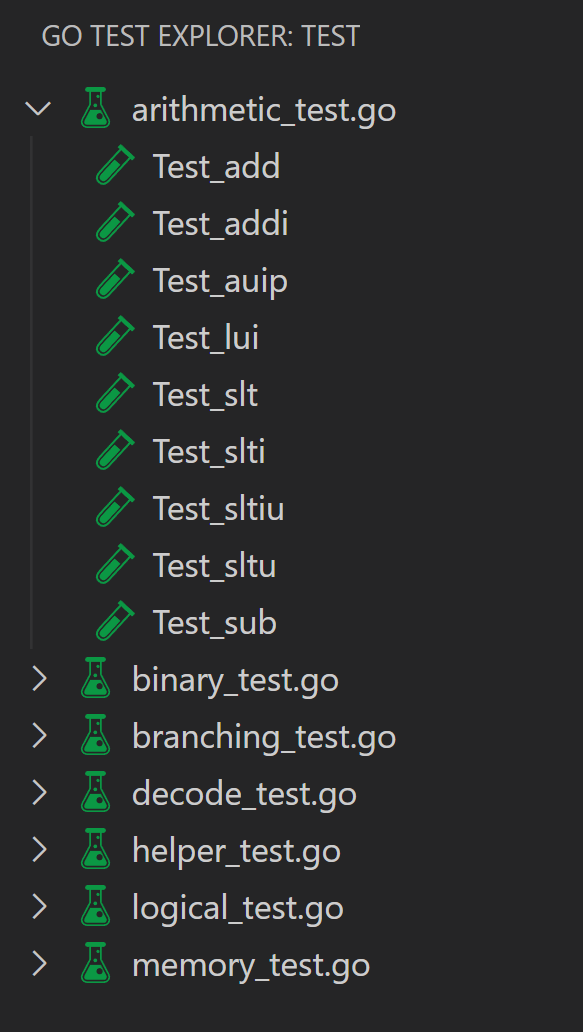
\includegraphics[width=0.4\textwidth]{images/test.png}
\end{wrapfigure}

\subsection*{Testing}
Simulator package is tested with test


Some text here and her and here
Some text here and her and here
Some text here and her and here
Some text here and her and here
Some text here and her and here



\begin{figure}[h]
\begin{minted}[linenos]{golang}
func Test_add(t *testing.T) {
    Reg[5] = 5
    Reg[6] = 3
    add(1, 5, 6)
    assert(Reg[1], 8, t)
}
\end{minted}
\end{figure}

\begin{wrapfigure}{r}{0\textwidth}
    \centering
\end{wrapfigure}
\newpage